% !Mode:: "TeX:UTF-8"
% 文字编码:UTF-8
\chapter{面向电视盒子的实时视频通话系统}
\label{chap:system}
在前面两章介绍的视频码率自适应算法和非对称差错保护算法部分,我们已经在实验中取得了良好的视频传输效果。为了在更加真实的环境中验证我们的算法,并使其发挥最大的应用价值,我们基于开源视频通话软件实现了一个面向安卓电视盒子和智能手机双平台、提供高清视频通话的软件,我们将其称为TVphone(TV based video phone)。该软件的目标是基于未来全面覆盖的家庭Wifi和公共Wifi 等信道,利用具有多媒体功能,提供的大屏幕、高清晰影像的电视盒子以及随时随地进行视频通话的智能手机两种平台,提供兼顾了通话效果和便利性的高清视频服务,并克服由高清视频大数据量以及无线网络质量差等对保障视频质量造成的困难。本章主要介绍TVphone 系统的整体设计模式、主要算法模块的实现框架和运行效果测试。


\section{背景介绍}
随着无线网络的覆盖日益广泛以及手机流量越来越廉价,人们日常生活休闲中对视频服务的需求量也越来越大,而这其中对人们生活方式改变最大的应该是通信方式从语音向信息量更丰富的视频通话转变。目前提供视频通话的应用如FaceTime、QQ、微信视频、Skype、环聊等使用率越来越高,一系列以此为基础的多媒体软件也快速涌现。

在底层传输方面,绝大部分实时视频服务都采用了RTP(Real-time Transport Protocol)实时传输协议。该协议提供了在互联网上传输实时数据(音频、视频等)所需要的基本功能,如时间戳同步、数据排序等。但该协议没有提供数据保护或传输质量保障功能,因此传输中一般还使用RTCP(Real-time Transport Control Protocol)用于传输质量监测、反馈等功能,从而实现基本的链路控制和数据保护。RTCP协议定时向发送方反馈当前网络的延迟、丢包率、网络抖动等网络基本信息,在发送端结合具体的码率自适应算法进行码率控制。在目前的视频通话应用中,主要使用了基于状态机的自适应算法,结合工程师的经验添加复杂的控制逻辑进行效果优化,而这一过程是没有理论分析支持的。另一方面,由于RTP协议不支持冗余保护,目前很多视频通话服务都没有丢包恢复功能,更不用说对冗余分配的优化,因此在信道质量较差的网络中往往播放效果很差。这也是我们前面两章的算法以及系统实现中主要解决的问题。

在本研究中,我们希望通过重新实现视频通话系统的底层传输模块,一方面利用我们的码率自适应算法,实现视频通话过程中的延迟可控,并通过理论分析有针对地提升码率调整的效果;另一方面,增加一个独立的FEC冗余保护模块,并结合冗余分配优化方案,在高丢包网络下保证稳定的视频质量。考虑到实时视频传输过程中涉及到的视频采集、编解码、播放以及传输过程中的连接建立、维护等功能实现起来都十分复杂并且已经有成熟的实现,而且这部分也不是本研究中关注的重点,因此我们选择了比较成熟的开源视频通话软件Linphone\cite{website:linphone}作为算法模块实现的基础。


    \subsection{Linphone项目框架}
    Linphone是一个开源视频通话软件,平台支持非常全面,包括Windows、MAC OSX、Linux、Android、iOS等。其核心模块为Liblinphone库,实现了除用户界面以外的所有Linphone功能,并且提供了丰富的用户接口,如音频、视频通话的发起、结束、设置等。Liblinphone库包含了三个功能模块,分别是:
    \begin{description}
        \item[Mediastreamer2] 流媒体处理,包括音、视频的采集、编解码等功能
        \item[oRTP] 负责流媒体传输,RTP和RTCP协议的具体实现
        \item[belle-sip] 提供SIP协议支持的库
    \end{description}
    以上所有Liblinphone的内容都采用纯C代码实现。在TVphone的开发中,我们主要关注包含视频处理的Mediastreamer2模块和负责视频传输的oRTP模块。

    \begin{figure}[htbp]
      \centering
      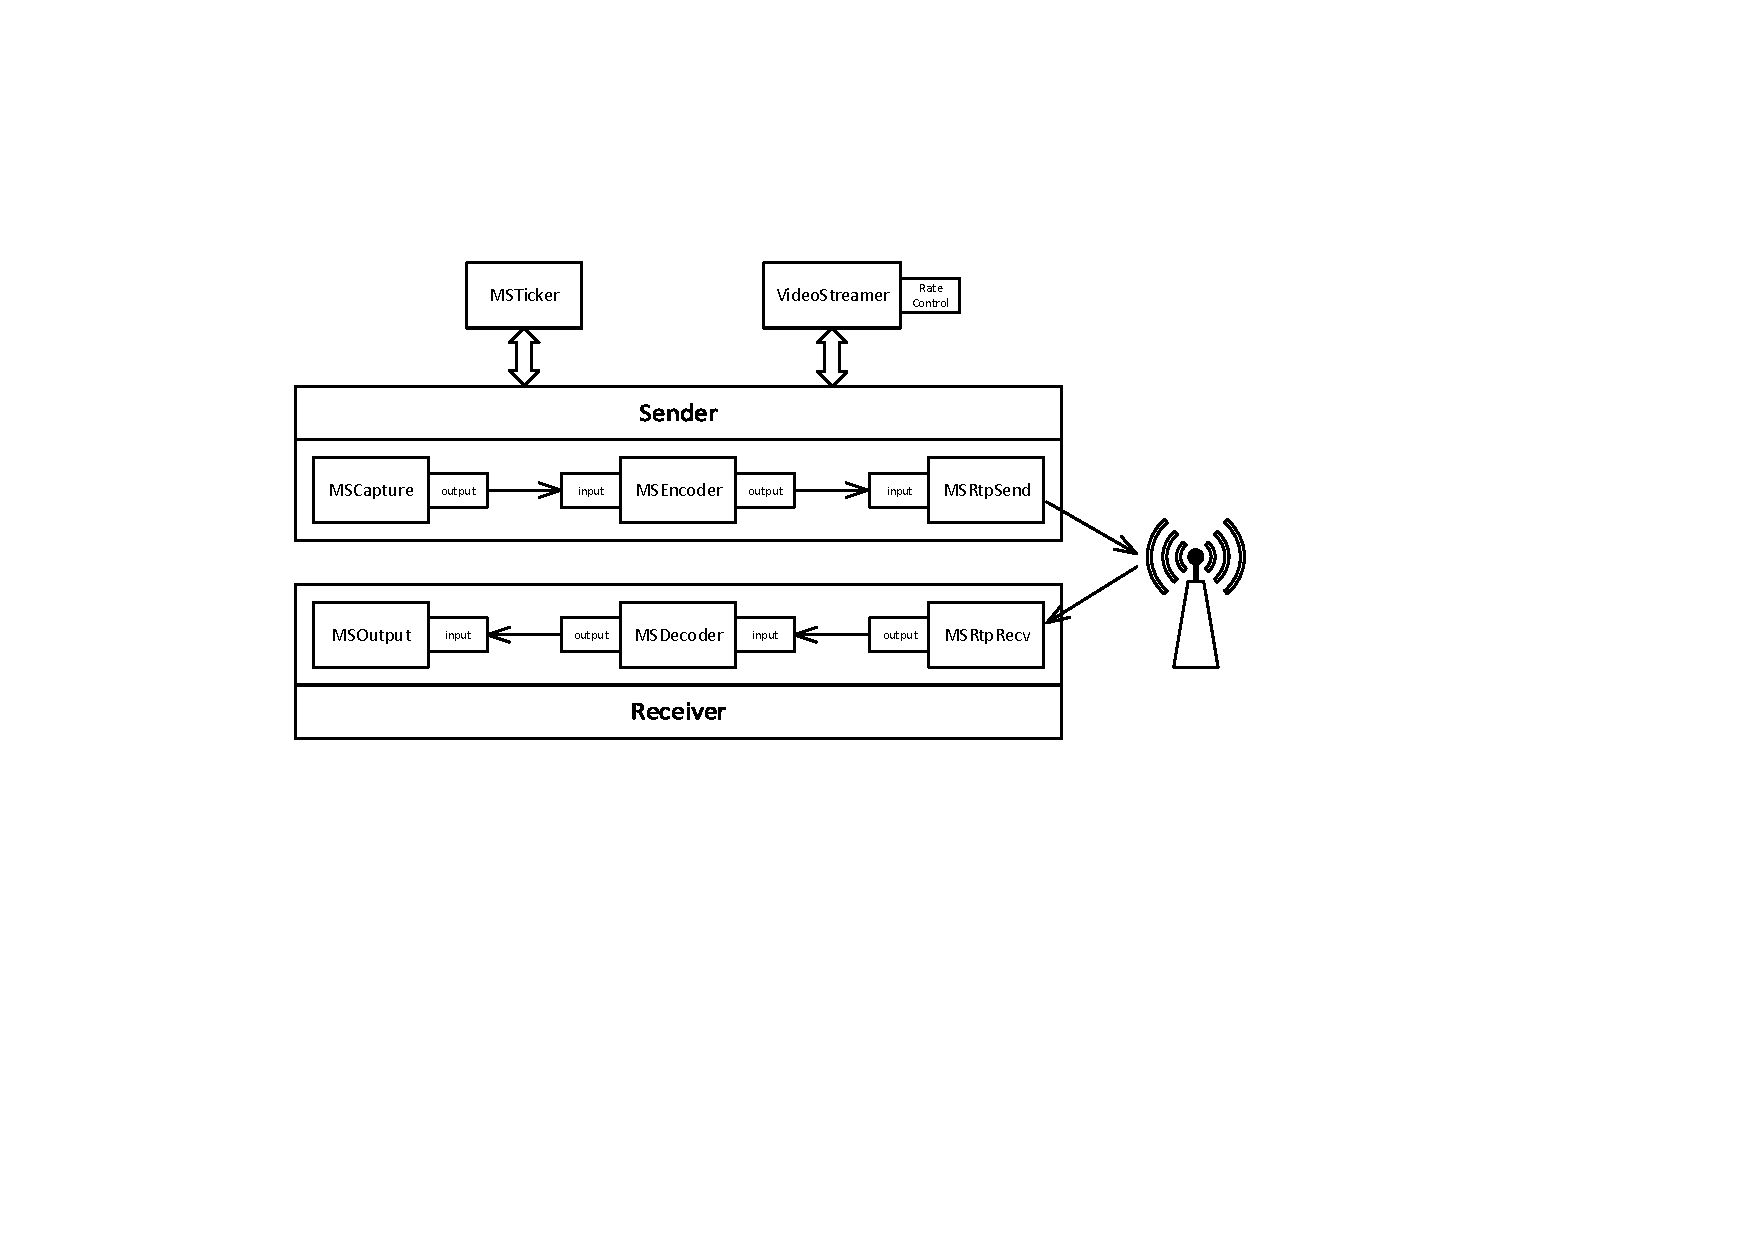
\includegraphics[width=0.9\textwidth]{linphone1.pdf}
      \caption{Liblinphone系统框架}
      \label{fig:linphone1}
    \end{figure}

    Liblinphone采用了模块化的设计模式,每一个功能模块实现为一个Filter数据结构,完成一项具体操作(视频采集、编码、封装等)。每个Filter都实现了统一的输入和输出接口,利用函数指针将需要的Filter组合起来即可完成整个服务过程,其基本框架如图\ref{fig:linphone1} 所示。在发送端,MSCapture完成视频数据的采集,原始视频数据进入MSEncoder进行压缩编码,编码后的数据在MSRtpSend完成RTP协议封装并通过网络链接向接收端发送。接收端MSRtpRecv接收到网络数据,对RTP数据包进行拆包得到视频数据,经过MSDecoder解码即可通过MSOutput播放视频画面。另外VideoStreamer是一个单独启动的Filter,完成网络信息的收集和反馈并以此为基础进行码率控制。注意到图中VideoStreamer附带的码率控制(Rate Control)模块是Linphone已经实现的码率控制协议,实现了一套较复杂的基于状态机的码率控制,但在后续实验中可以看到,其表现尚有较大提升空间。另外,上述过程通过在独立线程中启动的MSTicker 进行调度。以上所有Filter 都只定义了输入和输出信息的格式,因此可以根据需要随意替换其具体实现,如MSEncoder 可以实现为VP8 或H.264 等不同的视频编码格式。

    \subsection{RTP与RTCP传输协议}
    RTP(实时传输协议),顾名思义就是用来传输实时数据的,它作为因特网标准在RFC 3550\cite{jacobson2003rtp}中有详细说明。它为实时音、视频传输提供实时的传输服务,其中包括载荷类型标记、序列编号、时间戳和送达检测等。接收端可以利用RTP包头中的序列号和时间戳进行数据包的重排序和丢包检测。大部分应用将RTP建立在UDP协议之上,以利用其数据包校验、多地址发送等特性。需要注意的是,RTP本身并不提供任何机制保障数据包按时到达或其他传输质量保证,数据包可能发生丢包或乱序到达。

    RTCP为RTP数据流提供信道外控制。RTCP本身并不传输数据,而是定期在会话参加者之间传输控制数据。RTCP的主要功能是为RTP所提供的服务质量提供反馈。RTCP收集相关媒体连接的统计信息,如传输字节数,传输分组数,丢失分组数,jitter,单向和双向网络延迟等等,网络应用程序即可利用RTCP的统计信息来控制传输的品质,比如当网络带宽高负载时限制信息流量或改用压缩比较小的编解码器设置。

    Linphone中的oRTP模块就是对上述RTP和RTCP协议的封装,并实现了数据包的丢包检测,重排序等功能。我们的码率自适应算法也主要使用了RTCP协议所携带的网络信息进行码率控制。

\section{系统设计}


\subsection{设计框架}

\begin{figure}[htbp]
  \centering
  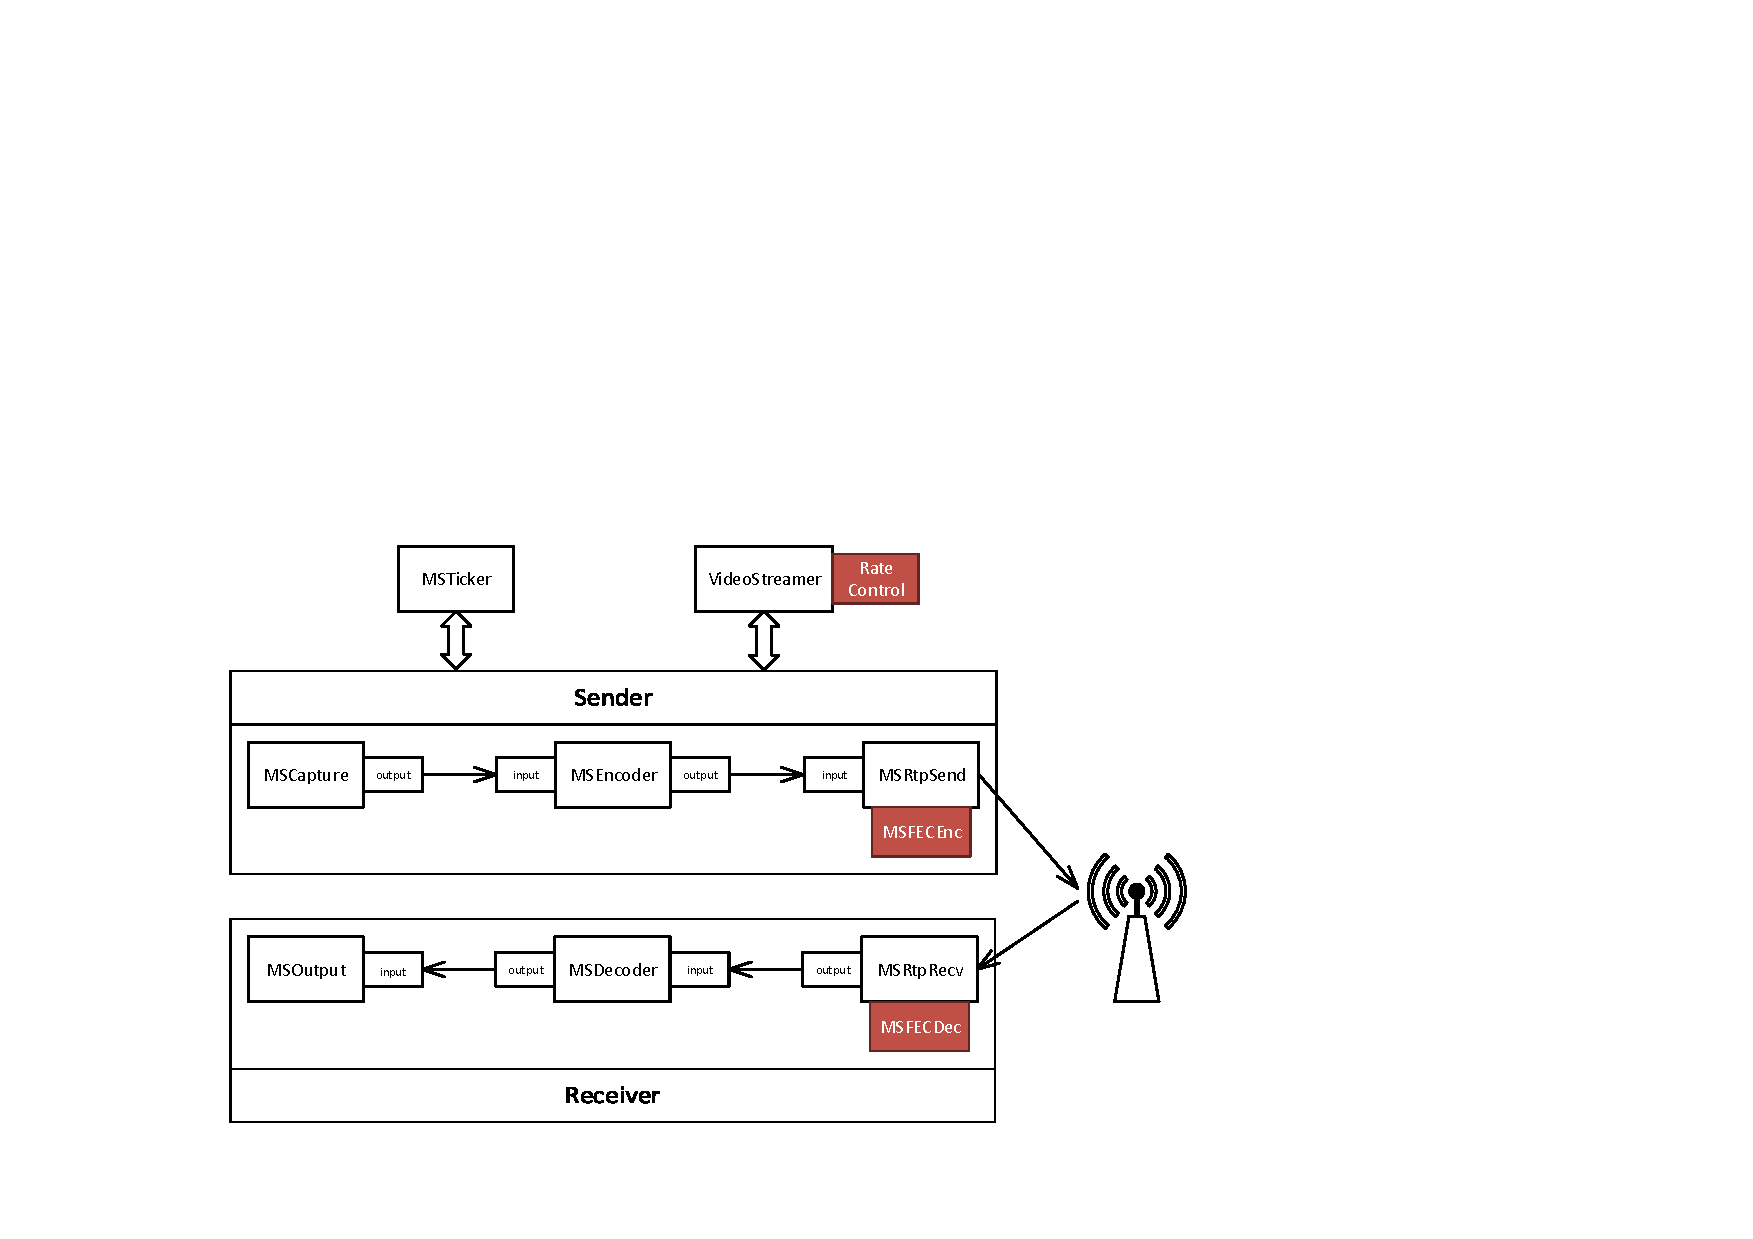
\includegraphics[width=1\textwidth]{linphone2.pdf}
  \caption{Liblinphone改进系统框架}
  \label{fig:linphone2}
\end{figure}

如上所述,在TVphone系统中,我们希望集中于码率自适应和差错保护两个模块的实现和优化,对于视频采集播放、编解码、RTP封装等操作直接沿用Linphone中的代码。基于上述Filter设计模式,我们设计出如图\ref{fig:linphone2}所示的改进系统框架。

一方面,我们沿用Linphone原有的码率控制框架,进行一些必要的改进之后植入了我们的码率自适应模块。我们在接收端通过一个网络探测模块获取网络状况信息并输入码率自适应模块,该模块输出相应的最优视频码率并通过RTCP协议发送给发送端,在发送端调用底层视频编码器接口改变输出视频的码率。

另一方面,根据原始LibLinphone 的MSRtpSend和MSRtpRecv模块设计,底层进行RTP包封装后直接发送数据到UDP网络层。为了实现冗余保护功能,我们在MSRtpSend 的输出端和网络链路之间增加了一个FEC 冗余编码模块 MSFECEnc,以及在MSRtpRecv 处理网络数据包之前增加了一个FEC 解码模块 MSFECDec,这两个模块分别作为RTP模块的附属功能单元进行FEC编解码操作。这样,所有发送到网络的RTP 数据包都添加了FEC 冗余数据,只要丢包数量低于FEC 解码的阈值,即可避免视频失真。


\subsection{码率自适应模块}
码率自适应是实时视频传输过程中最核心的控制模块,保证了视频通话服务在任何网络下都能顺利进行并获得相对较好的效果。我们设计的TVphone码率自适应模块主要采用了第\ref{chap:rate}章提出的延迟优化的实时视频码率自适应算法,针对实时视频的需求以排队延迟为输入,以低延迟和稳定高效的带宽利用为目标进行视频码率控制。

    \subsubsection{上层接口描述}
    \begin{lstlisting}[language=C]
int rc_process_rtcp(MSQosAnalyzer *objbase, mblk_t *rtcp);
    \end{lstlisting}
    
    码率自适应模块对上层提供的接口只有一个函数\lstinline!rc_process_rtcp!,该函数以RTCP包为输入,完成网络状态信息收集、码率计算、定时反馈等任务。其输入 \lstinline!objbase! 指向码率自适应模块的内存实体,记录码率自适应算法的设置、历史信息等; \lstinline!rtcp! 指向接收到的RTCP包。输出为代表函数执行状态的整数代码。函数在系统收到携带网络状态信息的RTCP包时被调用。

    \subsubsection{模块介绍}
    \begin{figure}[htbp]
      \centering
      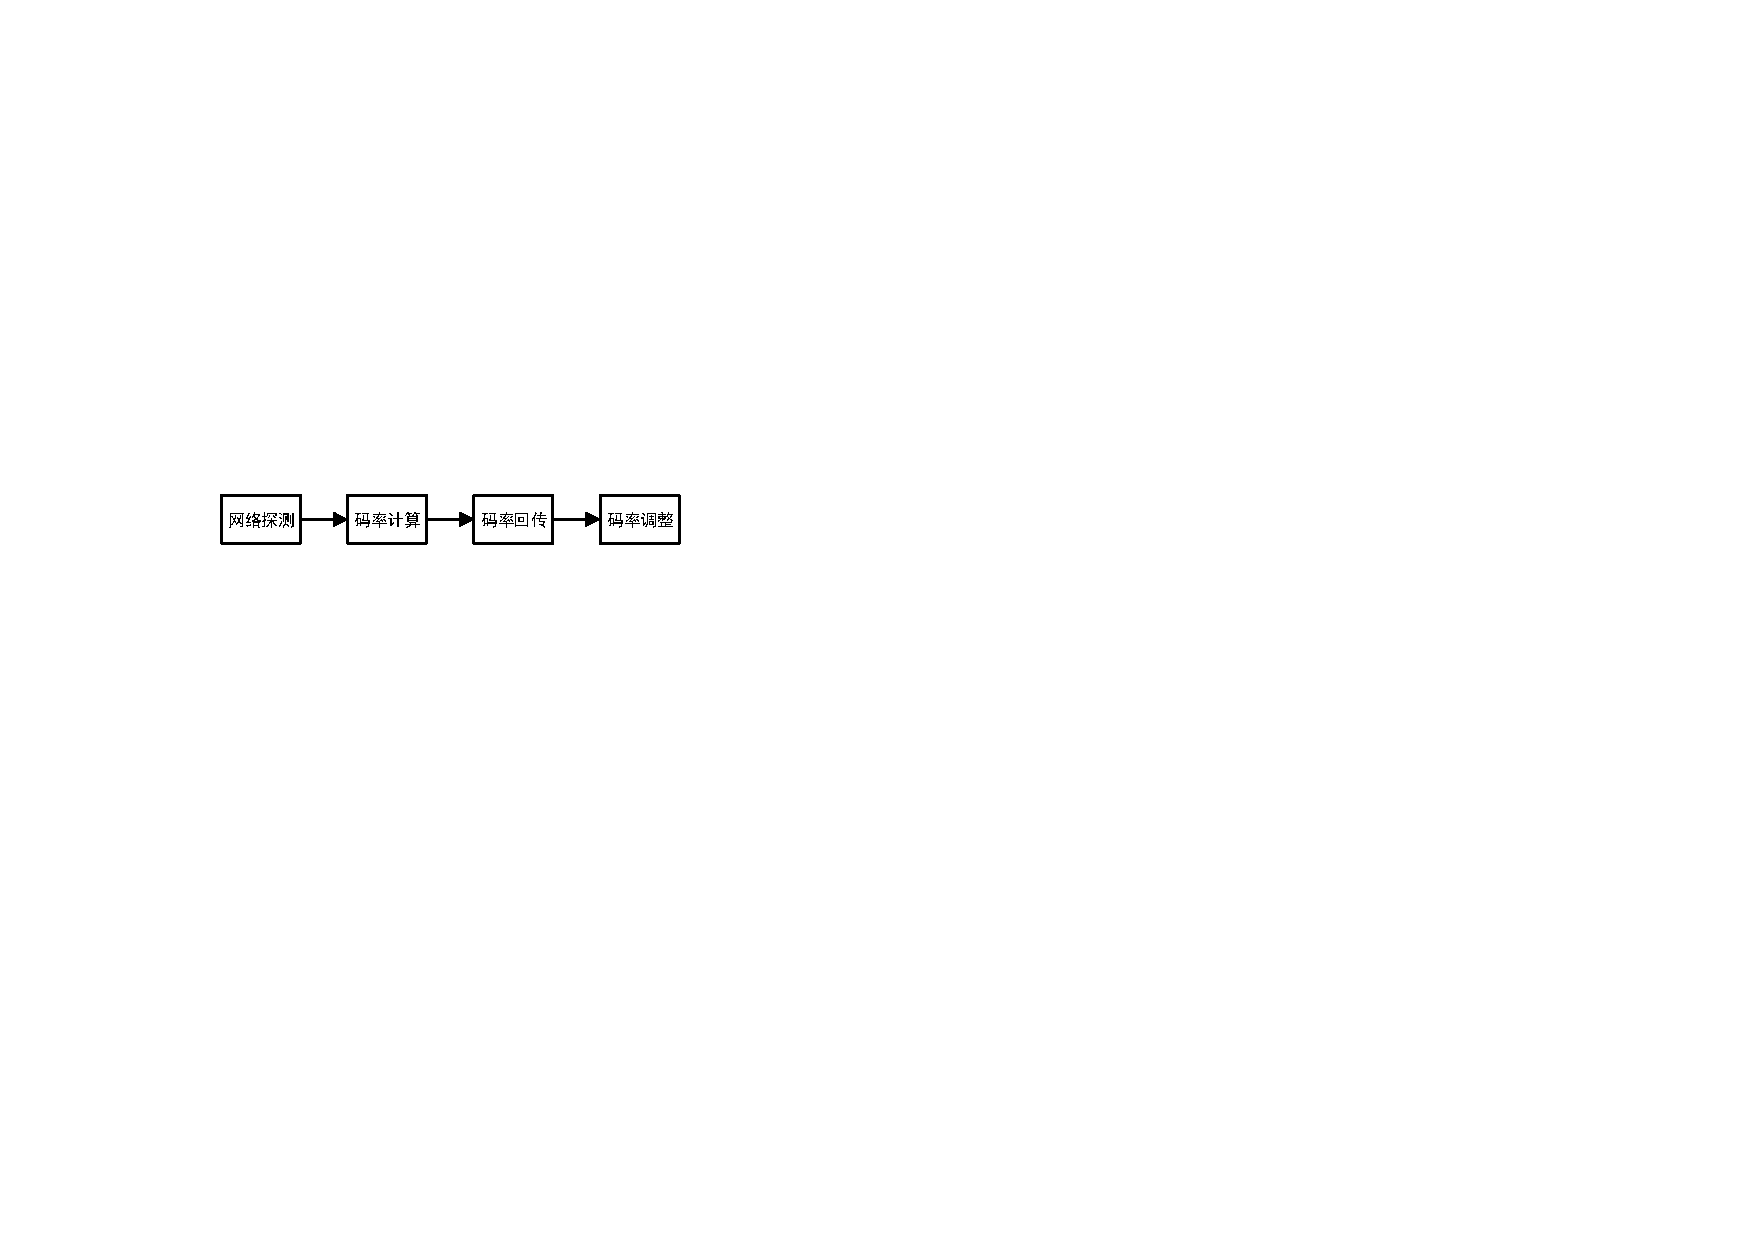
\includegraphics[width=0.8\textwidth]{rate_control.pdf}
      \caption{码率自适应模块设计框架}
      \label{fig:rate_control_arch}
    \end{figure}

    如图\ref{fig:rate_control_arch}所示,码率自适应模块的主要功能单元包括网络探测、码率计算、码率回传和码率调整四部分。

    ``网络探测''单元为码率自适应算法提供必要的网络运行状态参数,在我们的算法中主要用到排队延迟。在第\ref{chap:qd_calc}节中,我们已经给出了利用单向延迟计算排队延迟的方法,因此网络探测模块需要提供单向延迟的探测。为了探测网络的延迟,发送端每隔100ms发送一个RTCP探测包并标记发送时刻的时间戳,接收端收到该RTCP包即可利用发送和接收的时间差计算单向延迟、最小单向延迟,进而根据式\ref{eq:qd}计算排队延迟。另外,网络探测模块还根据收到RTP包的序列号统计网络丢包率,以供极端情况下的码率调整和差错保护。

    ``码率计算''单元是运行在视频接收端的功能单元,其根据网络探测输入的延迟和丢包率信息,套用第\ref{chap:rate}章算法计算目标码率并提交给``码率回传''单元反馈给发送端。将码率计算单元设置在接收端主要有两点考虑:
    \begin{enumerate}
        \item 视频传输过程中,排队延迟、丢包率等网络参数的统计都在接收端完成,回传目标视频码率的通信量明显低于回传全部网络参数所需要的通信量。
        \item 系统运行过程中,接收端网络参数的采集频率可以很高。码率计算在接收端进行,更频繁地计算目标码率值,并根据这一值的变化情况动态地选择更加合理的回传频率,以优化系统反应速度和带宽占用。
    \end{enumerate}
    视频码率的调整速率对视频通话系统的很多方面都有影响。如果码率调整间隔太大,会造成网络拥塞状况得不到及时解决,出现较大的延迟波动;单次调整变化过大,对用户体验造成一定影响。而如果码率调整太频繁,会造成视频编码器负载增大;回传次数增多,网络负载增加等问题。通过实验测试,我们选择了500ms作为码率回传单元回传码率的默认时间间隔。另外如果两次计算的目标码率变化超过一定阈值,则会立刻发送该目标码率以避免网络拥塞。

    码率调整单元直接调用视频编码器Filter提供的接口进行设置,由具体的VP8、H.264等编码器实现视频输出码率的控制。需要注意的是,大部分视频编码器并不能完全将输出码率固定在一个准确的值,而是会在一定范围内波动并尽量使平均码率接近目标值。这一点也给实时视频的码率自适应策略带来一定的困难。


\subsection{差错保护模块}
差错保护是视频通话系统的可选模块,以增加带宽占用为代价提供一定的丢包恢复能力。在无线网络场景下,现有技术已经实现了非常高的峰值带宽,然而由于传输信道的局限,仍然存在一定的丢包情况。因此无线网络下应用差错保护成为一种性价比很高的提升视频通话效果的方案。基于无线网络通信的需求,我们在TVphone系统中添加了一个独立的差错保护模块,并用第\ref{chap:fec}章提出的非对称差错保护算法对保护效果进行了优化。该差错保护模块的设计框架如图\ref{fig:fec_arch}所示。

    \subsubsection{上层接口描述}
    差错保护模块提供与FEC编解码相关的接口供oRTP模块调用,其主要接口如下:
    \begin{lstlisting}[language=C]
int fec_set_rate(MSFecDriver *obj, int block_size, int fec_rate);
int fec_outgoing_rtp(MSFecDriver *obj, mblk_t *rtp);
int fec_incoming_rtp(MSFecDriver *obj, mblk_t *rtp);
int fec_incoming_rtcp(MSFecDriver *obj, mblk_t *rtcp);
    \end{lstlisting}
    
    其中 \lstinline!fec_set_rate! 可以动态调整差错保护的平均冗余率,在系统初始化时调用,也可以在系统运行中根据网络状态调用该函数修改冗余率。当发送端 MSRtpSend 模块准备发送RTP包时,首先调用 \lstinline!fec_outgoing_rtp! 对RTP包进行缓存、FEC编码并发送FEC数据包(通过RTCP协议封装)。 当接收端 MSRtpRecv 模块收到RTP包或携带冗余数据的RTCP 数据包时,分别调用 \lstinline!fec_incoming_rtp! 和 \lstinline!fec_incoming_rtcp! 进行数据缓存、FEC解码并恢复丢失的RTP数据包。

    \subsubsection{模块介绍}
    \begin{figure}[htbp]
      \centering
      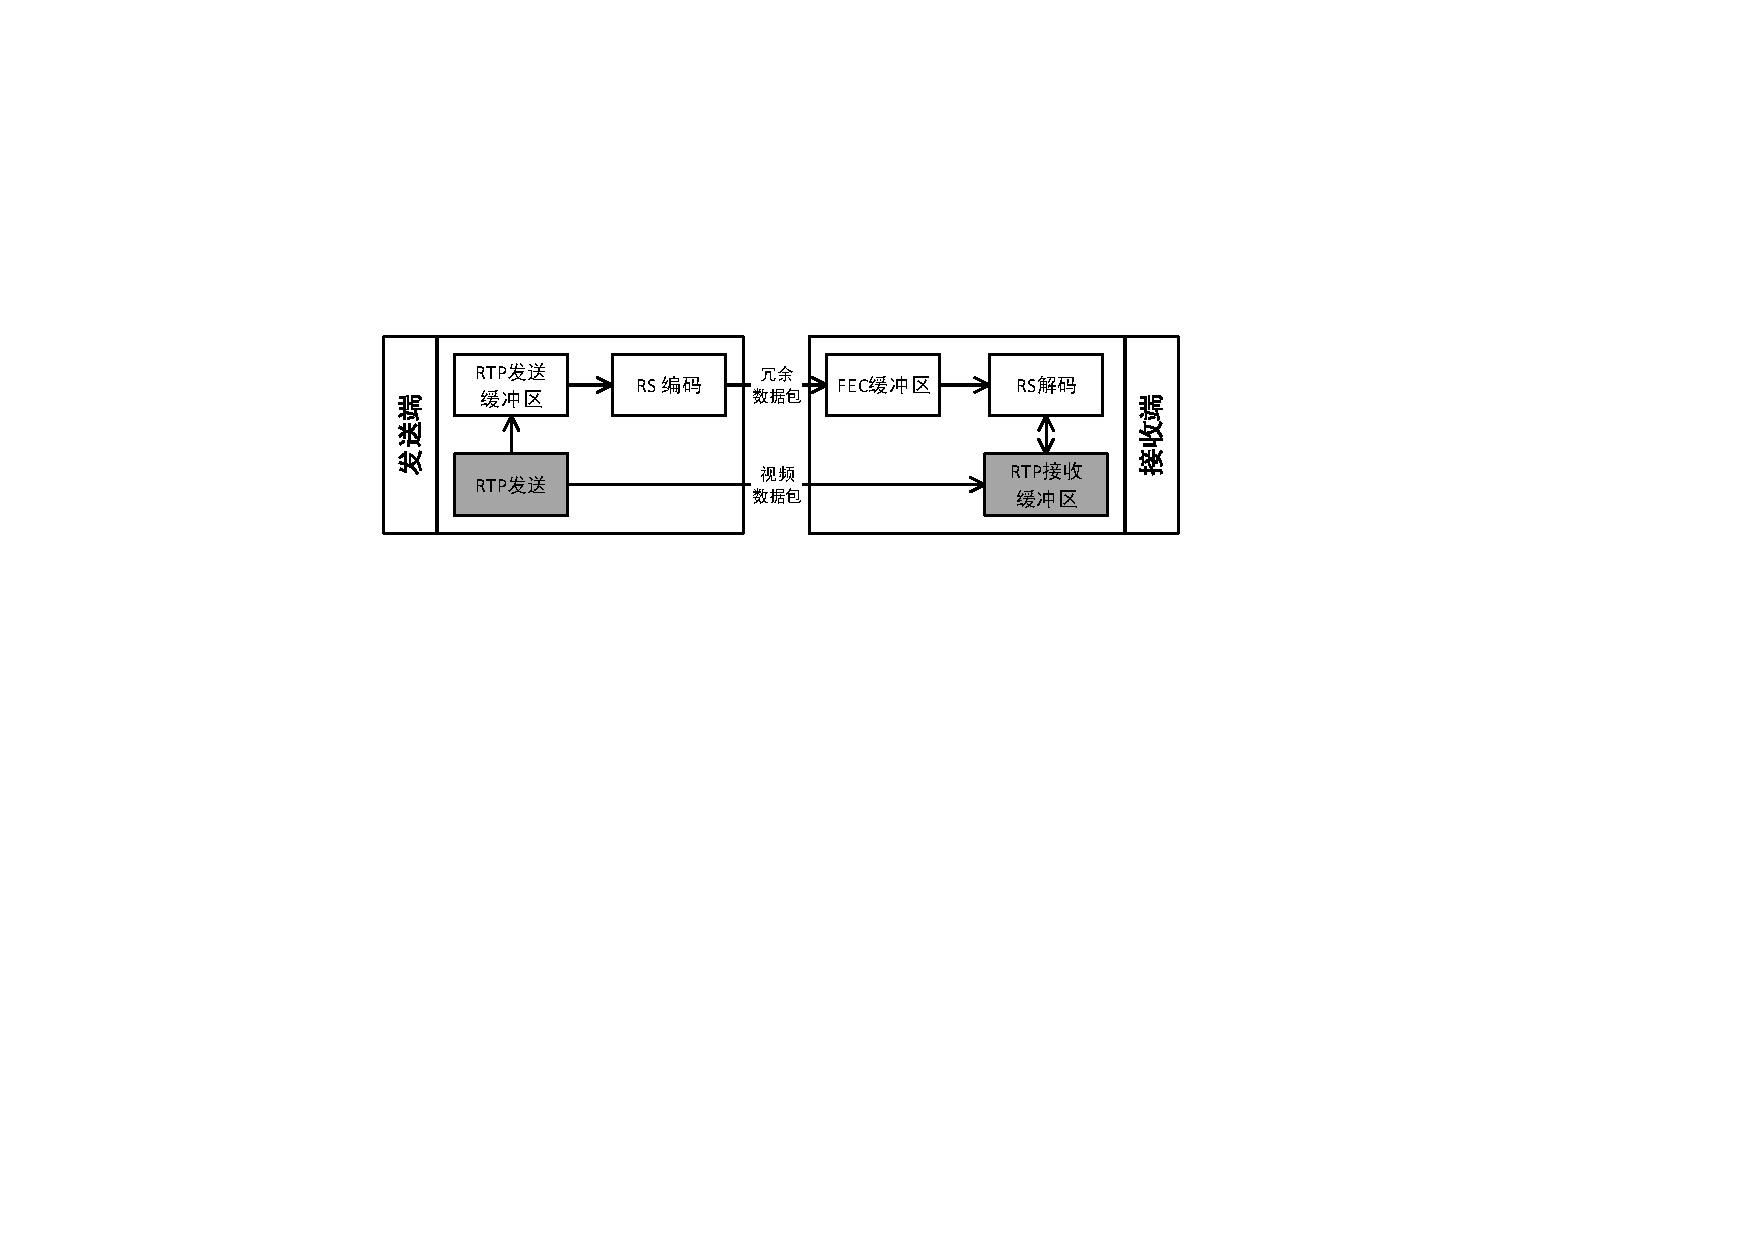
\includegraphics[width=1\textwidth]{fec.pdf}
      \caption{差错保护模块设计框架}
      \label{fig:fec_arch}
    \end{figure}

    图\ref{fig:fec_arch}中灰色单元为Liblinphone中的原生功能单元\footnotecircle{其中接收端``RTP缓冲区''单元进行了一些修改以适应扩展窗口编码要求},均实现于oRTP中,完成RTP 协议的部分功能。具体来说,底层视频编码器产生的数据经过oRTP 的封装形成RTP 包,通过``RTP发送''单元经UDP等网络层到达接收端。在负责接收的oRTP部分维护了一个``RTP 缓冲区'',用于缓存还未用于视频解码的RTP 包,并根据时间戳对RTP 包进行排序。当然由于实时视频传输的播放延迟非常小,因此这个RTP缓冲区内通常只缓存了很少的数据包。

    根据第\ref{chap:fec}章的描述,我们在差错保护模块采用了比较成熟的Reed-Solomon编码(RS编码),并使用了Github上的一个实现了Reed-Solomon编码的开源库longhair\cite{website:longhair} 作为底层编码单元。RS编码具有$RS(N,K)$编码格式,即每个编码块对$K$个RTP包进行冗余编码生成$N-K$个FEC校验包,在接收端只要接收到该编码块中的任意$K$个包,就能通过对编码块的解码完全恢复丢失的RTP包。因此在我们的差错保护模块中,发送端需要对待编码的编码块中的RTP包进行缓存,接收端则需要对接收到的RTP包和校验包进行缓存以备解码。因此在差错保护模块中包含了发送端和接收端的``RTP缓冲区''以及接收端的``FEC缓冲区''共三个缓冲区,而其中接收端的``RTP缓冲区''沿用了oRTP模块中的实现。

    发送端的``RS编码''和接收端的``RS解码''单元分别完成RS编码和解码过程。其中RS编码的输入为RTP缓冲区中的RTP包,编码结束后得到的冗余包经过RTCP协议发送到接收端。接收端以``RTP缓冲区''中的RTP包和``FEC缓冲区''中的校验包为输入,如果发现丢包并且满足$RS(N,K)$的解码条件,则进行解码恢复丢失的RTP包。这些恢复的RTP包也被放入``RTP缓冲区''等待下一步的视频解码。在RS编码过程中,还涉及到编码块的组织、冗余分配优化、编解码效果优化等实现细节,将在下节详细说明。

    \subsubsection{扩展窗口RS编解码实现}
    \begin{figure}[htbp]
      \centering
      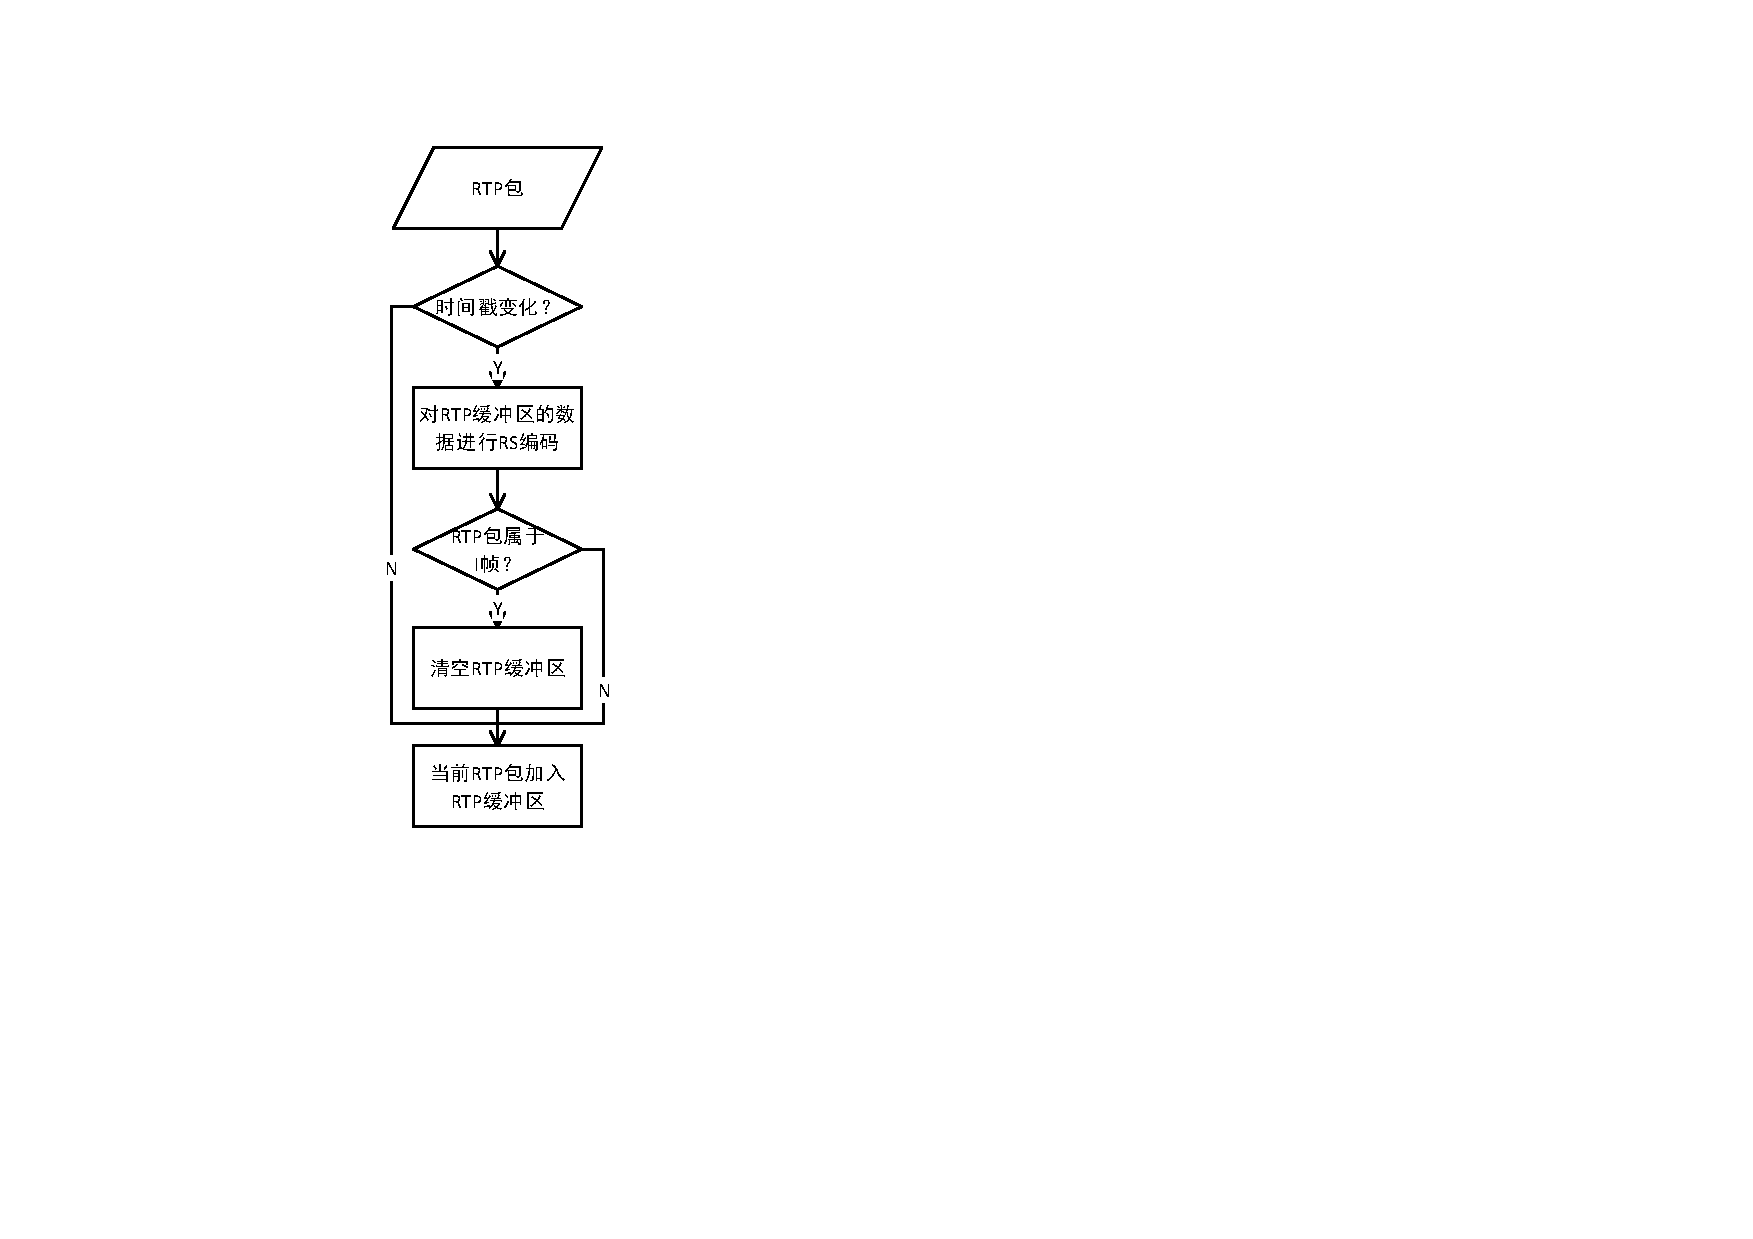
\includegraphics[width=0.25\textwidth]{fec_enc_seq.pdf}
      \caption{扩展窗口RS编码流程图}
      \label{fig:fec_enc_seq}
    \end{figure}

    由于我们的差错保护模块采用了基于扩展窗口的RS编码框架,在发送端RTP缓冲区的使用上与传统FEC编码过程有一定差别,编码过程也需要进行修改,发送端编码的流程图如图 \ref{fig:fec_enc_seq} 所示。当新的RTP包产生并发送到网络的同时,它的一份拷贝进入发送端的``RTP缓冲区''并触发RS编码模块的处理流程。首先RS编码器检查当前RTP包的时间戳与上一个RTP包是否发生变化。如果时间戳没有变化,说明他们属于同一视频帧,由于我们的编解码过程都以视频帧为边界(否则,若同一视频帧的数据包被分割在不同编码块,将会引入额外播放延迟),可以直接将当前RTP包加入RTP缓冲区。如果时间戳发生了变化,说明上一个视频帧的所有RTP包均已缓存,这时RS编码器以FEC缓冲区内的所有数据包为编码块进行RS编码,并发送生成的校验包。另外,如果当前RTP包属于I帧,说明我们已经处理完了一个GOP,需要重新开始扩展窗口过程,此时清空当前缓冲区。无论是否清空缓冲区,都需要将当前RTP包加入RTP缓冲区以备下一轮编码。

    \begin{figure}[htbp]
      \centering
      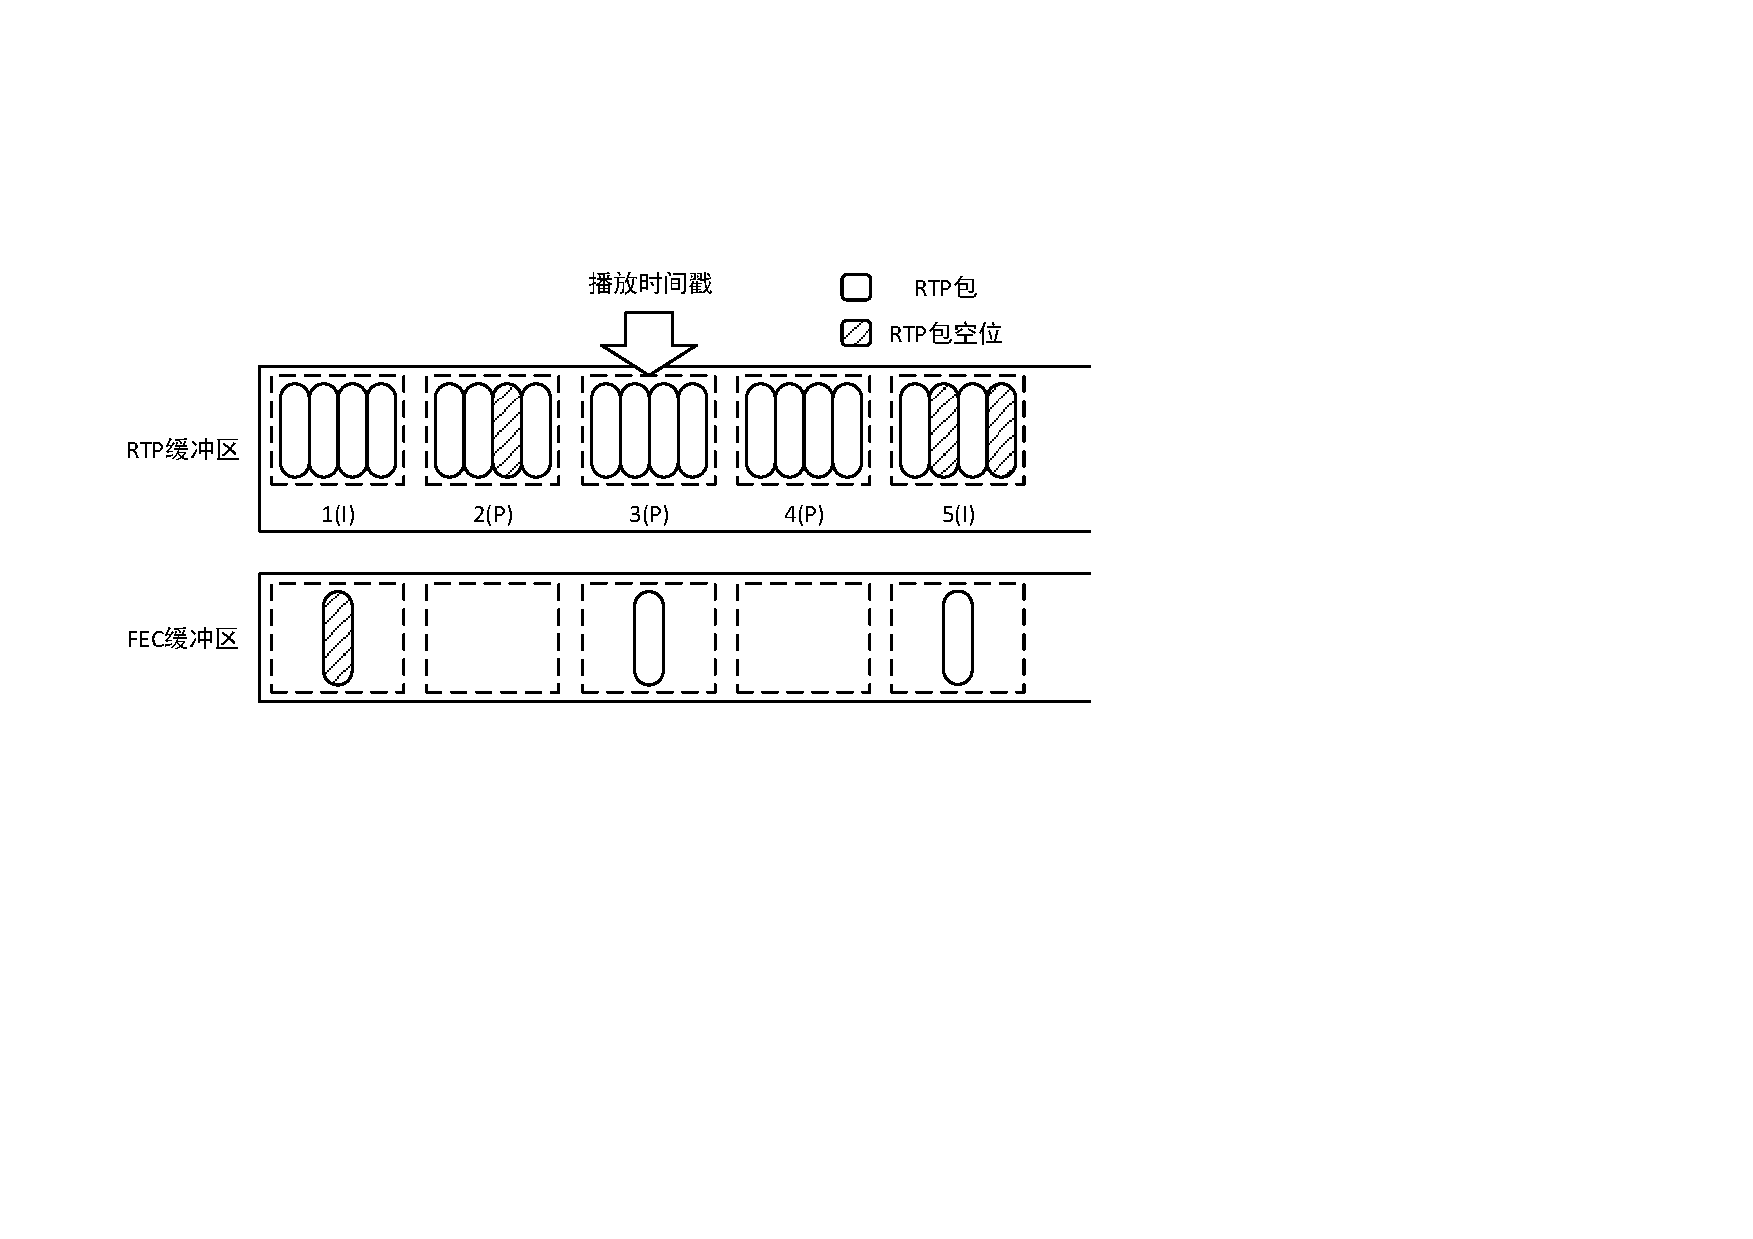
\includegraphics[width=0.9\textwidth]{fec_dec_buf.pdf}
      \caption{扩展窗口RS编码流程图}
      \label{fig:fec_dec_buf}
    \end{figure}

    在接收端,oRTP模块根据当前视频播放时间戳从RTP缓冲区中取出时间戳小于播放时间戳的所有RTP包,输出到后续视频解码模块进行解码和播放。为了方便描述,我们在图\ref{fig:fec_dec_buf}中给出了某一播放状态下的RTP缓冲区和FEC缓冲区状态,以及播放时间戳位置。如图所示,接收端的两个缓冲区中保存了当前待播放视频帧所在GOP的所有视频帧的数据包(图中1/5为I帧),及其之后的所有数据包。当播放时间戳到达第3帧并试图取RTP包时,首先对1-3帧组成的编码块进行解码,此时第2帧中丢失的RTP包可以被恢复,并将第2 帧的解码图像在解码器的参考缓冲区中更新,此时RS解码过程结束。值得注意的是,如果没有扩展窗口编码框架对第2帧的恢复,则当前GOP中的2-4帧都将无法解码,而通过这一框架使得3/4帧都得以解码播放。

    \subsubsection{冗余率和冗余分配优化}
    如果系统冗余率明显超出了纠正丢包所需的比例,会有大量冗余包得不到利用而造成网络带宽的浪费;而如果冗余率过低,又会造成大量丢包无法恢复,通话质量得不到保证。为了尽可能使冗余率适应网络需求,我们增加了一个简单的冗余率自适应功能。即如果网络丢包率连续三次高于 $5\%$ 则提高一档冗余率,如果网络丢包率连续三次低于 $1\%$ 则降低一档冗余率。经测试这一简单策略可以较好地实现网络变化时的冗余率自适应。
    
    针对第\ref{chap:fec}章中提出的冗余分配优化算法,我们需要根据当前网络的丢包率以及当前视频GOP中不同位置视频帧的特性计算合理的冗余分配方案。如果对于每个GOP都重新计算,将会严重增加客户端的计算负载,并且实时性也无法得到满足。因此我们每隔1分钟采样一次当前平均丢包率和GOP的视频帧特性,通过算法\ref{al:hc}计算最优冗余分配,并在下一次采样计算前的所有RS 编码中使用这一分配策略。


\subsection{面向电视盒子的界面优化}
基于上述对视频通话服务核心模块的增改,为了能够进一步体现高质量视频传输的效果并更好地服务于视频通话的需求,我们为TVphone设计了一套面向电视盒子的交互界面。通过这一界面,用户可以使用遥控器进行操作,直接在电视屏幕上实现视频通话,获得更好的用户体验。本章简要介绍其中几个主要界面的设计和实现。

\begin{figure}[htbp]
  \centering
  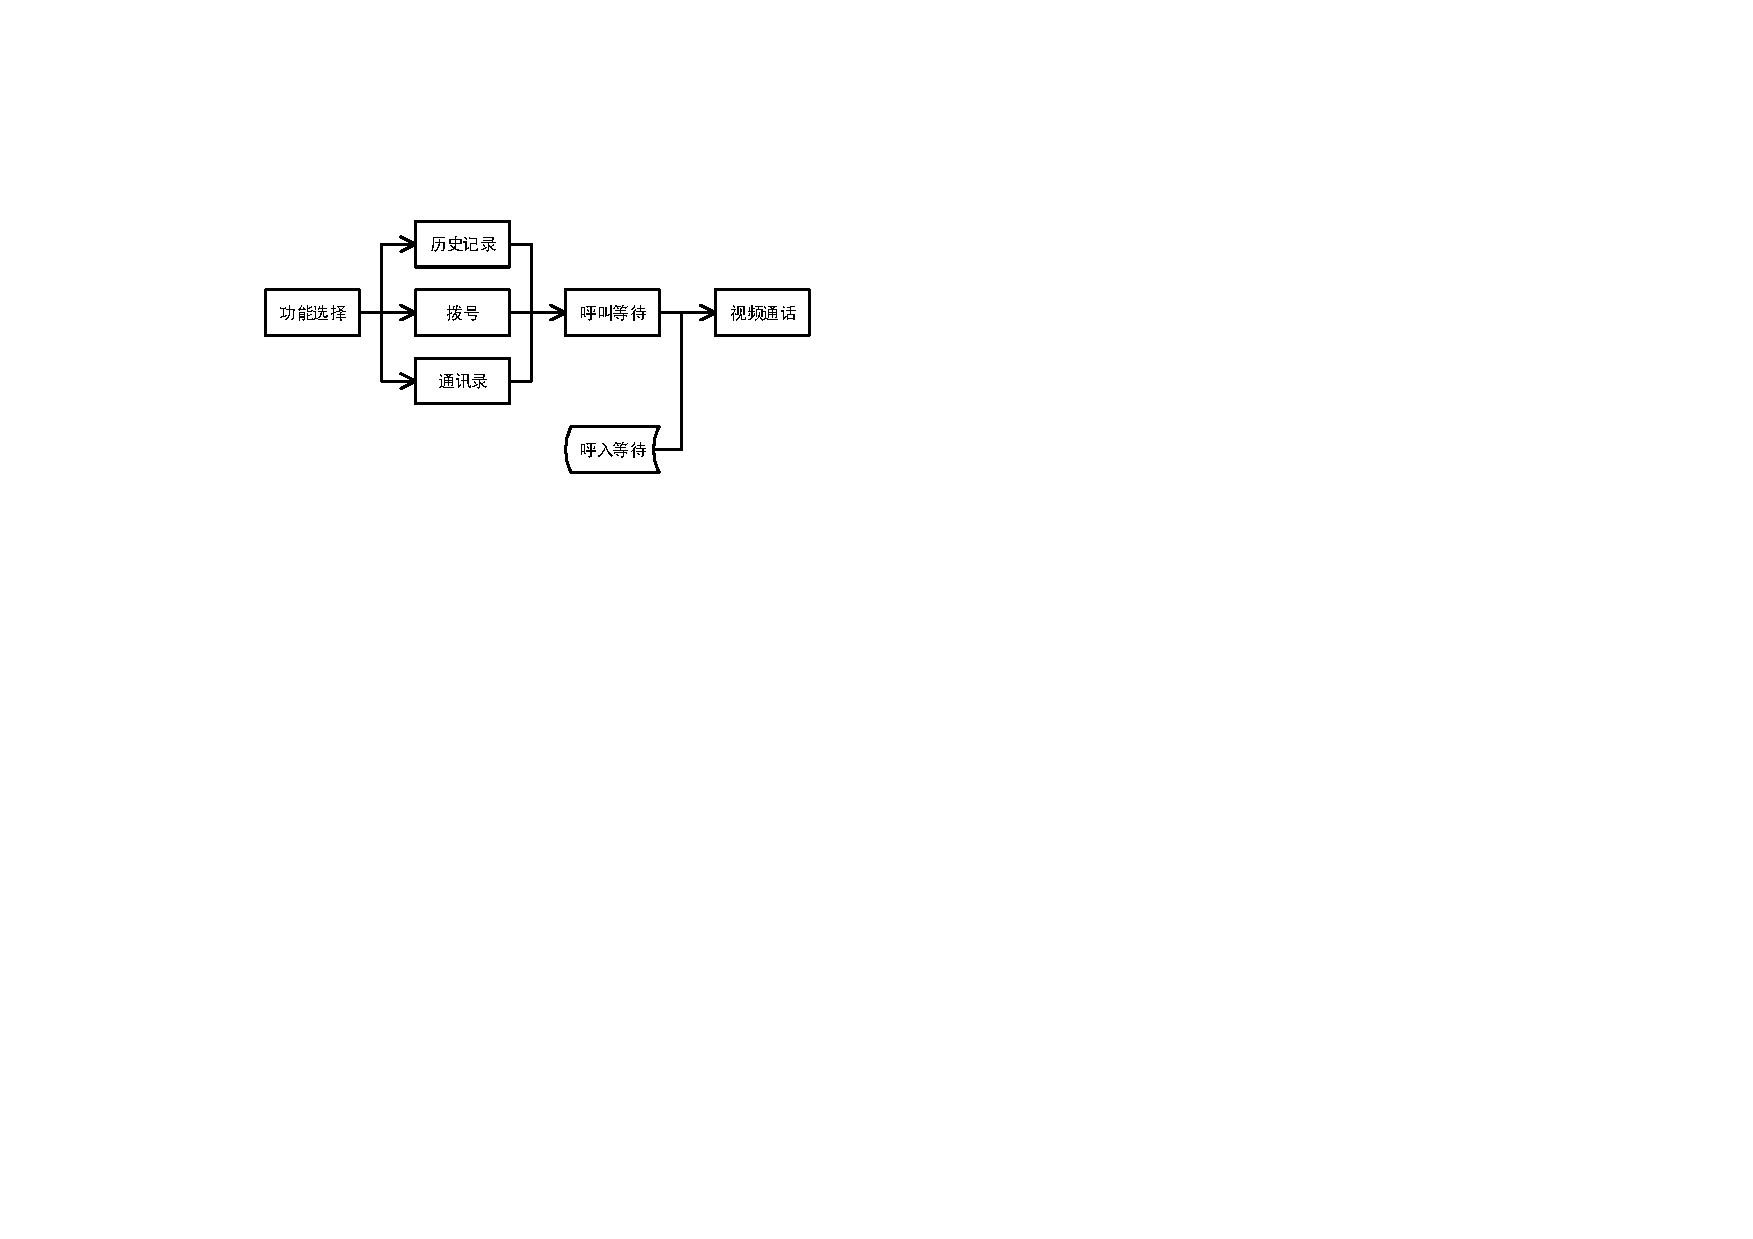
\includegraphics[width=0.7\textwidth]{ui_logic.pdf}
  \caption{页面跳转逻辑}
  \label{fig:ui_logic}
\end{figure}

本TVphone视频通话系统的主要页面跳转逻辑如图\ref{fig:ui_logic}所示。应用启动后,首先出现功能选择界面\ref{fig:ui_main},用户可以选择的功能包括:历史记录界面查看最近的联系人并可以直接拨号;拨号界面\ref{fig:ui_call}通过输入对方的联系方式发起呼叫;通讯录界面\ref{fig:ui_contact}则记录了用户主动保存的联系人。在上述三个界面均可以方便地发起视频通话请求,进入呼叫等待界面等待对方接通。同时,软件在后台对呼入请求进行监听,发现呼入请求后转到呼入等待界面\ref{fig:ui_incall}。当通话双方均做好准备后,就可以打开视频通话界面开始高清视频通话。

\begin{figure}[htbp]
  \centering
  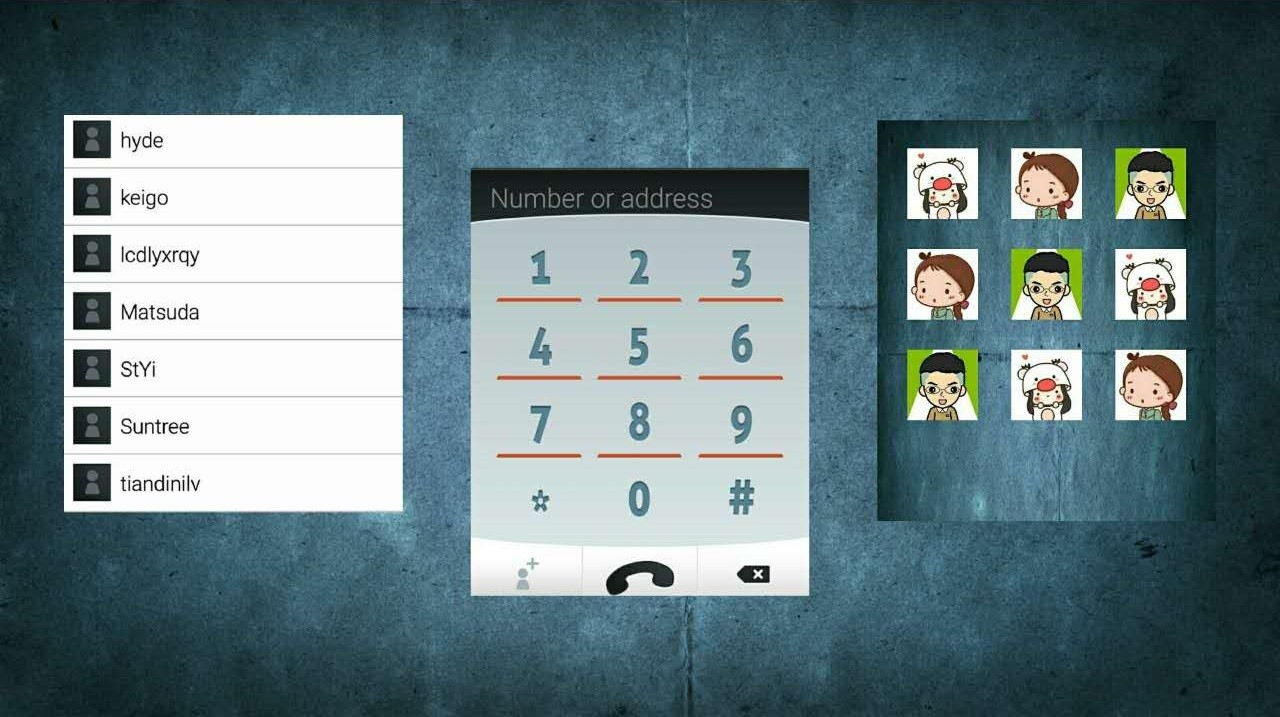
\includegraphics[width=0.6\textwidth]{ui_main.jpg}
  \caption{功能选择界面}
  \label{fig:ui_main}
\end{figure}

\begin{figure}[htbp]
  \centering
  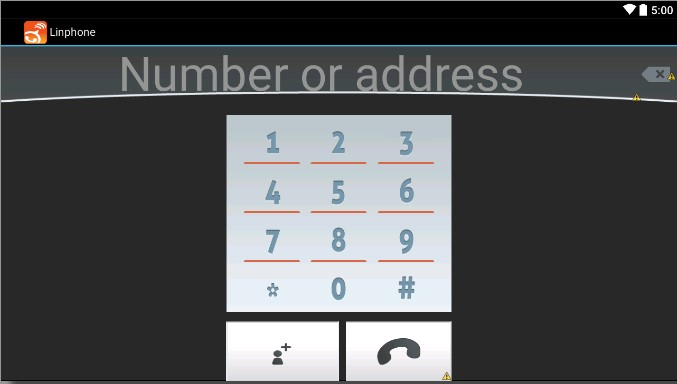
\includegraphics[width=0.6\textwidth]{ui_call.jpg}
  \caption{拨号界面}
  \label{fig:ui_call}
\end{figure}

\begin{figure}[htbp]
  \centering
  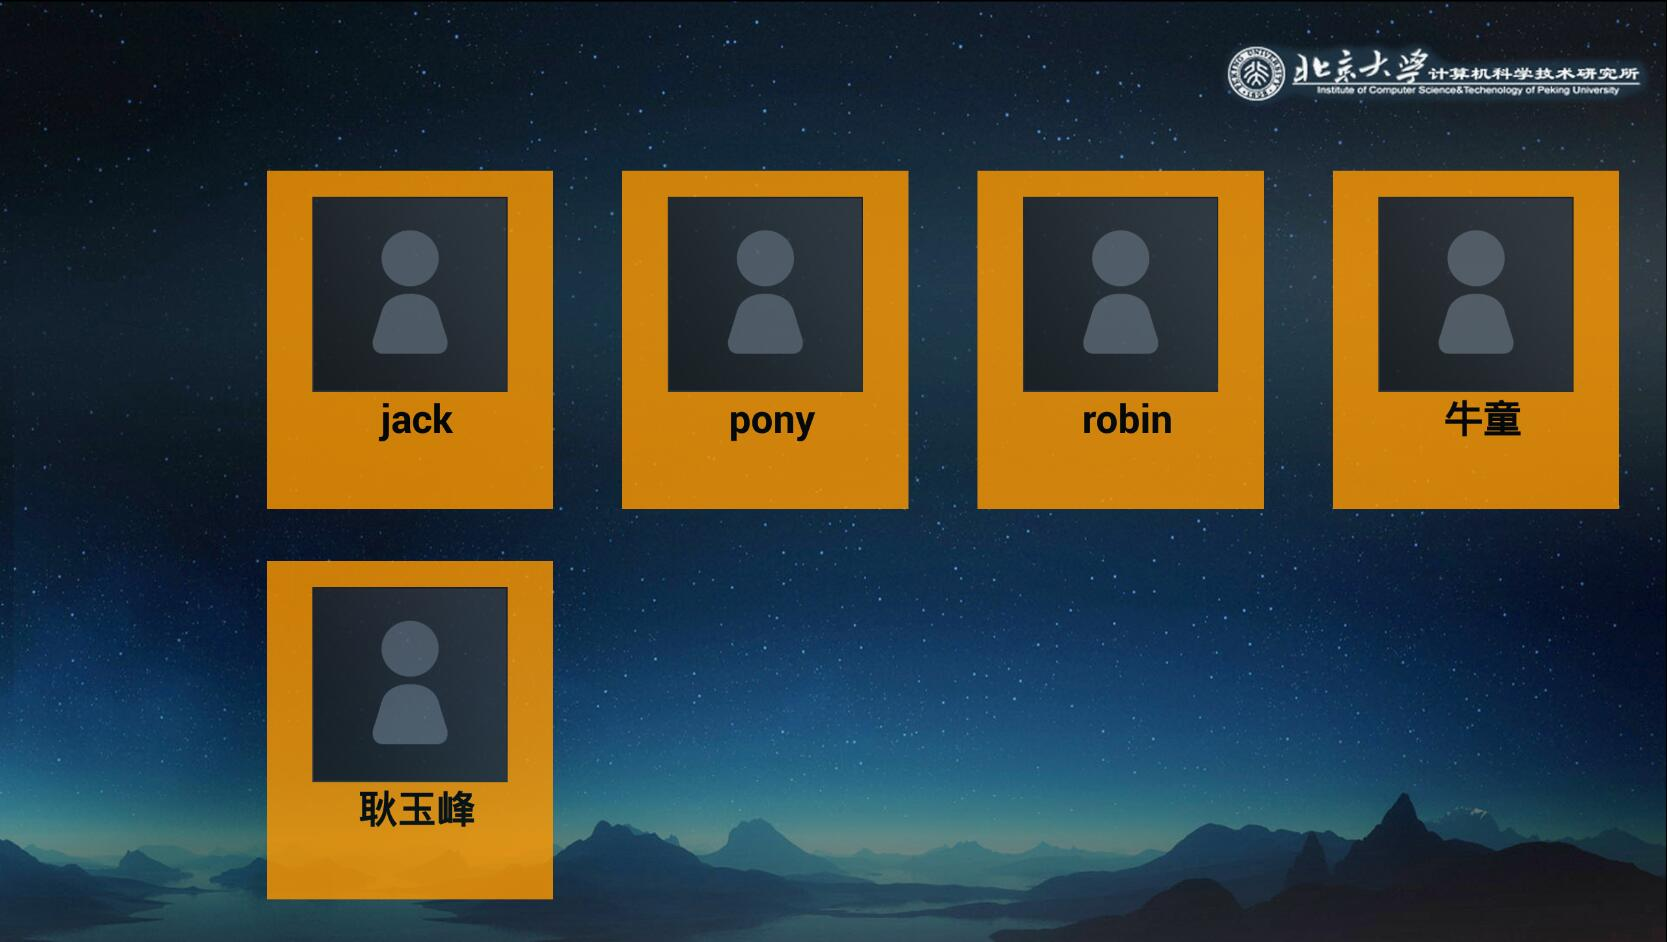
\includegraphics[width=0.6\textwidth]{ui_contact.jpg}
  \caption{通讯录界面}
  \label{fig:ui_contact}
\end{figure}

\begin{figure}[htbp]
  \centering
  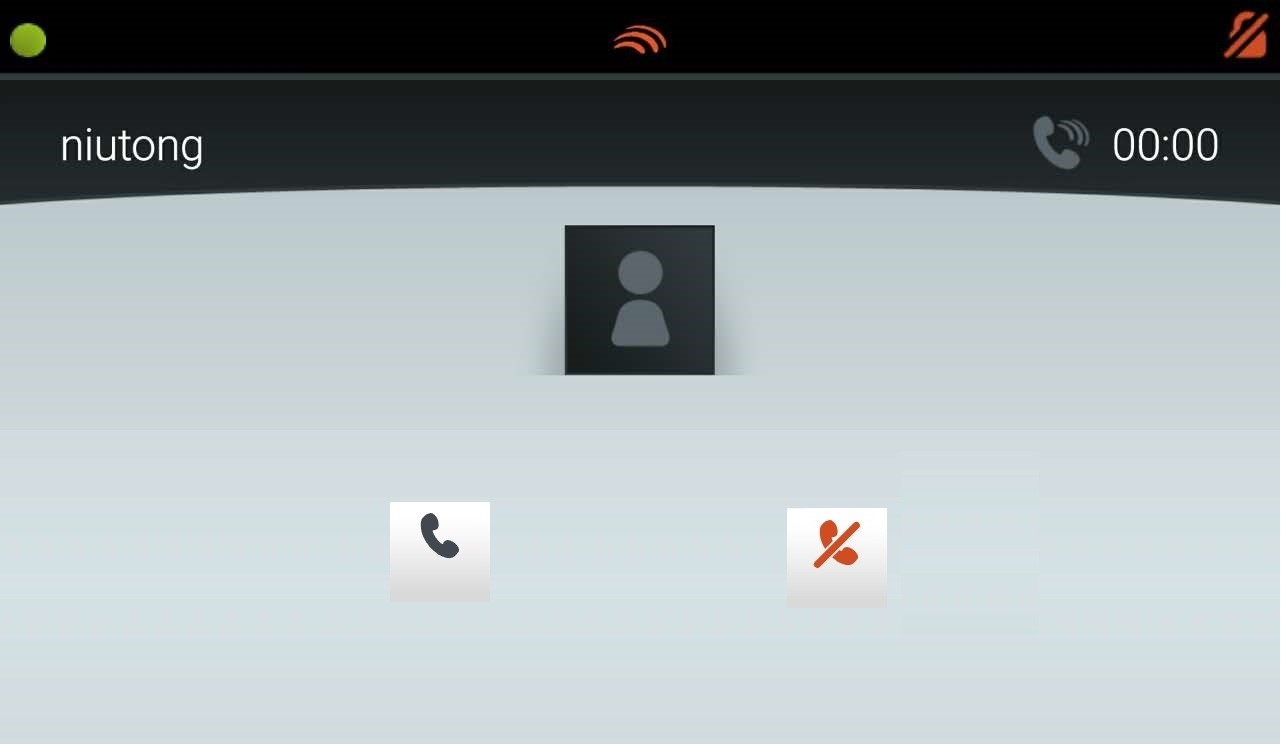
\includegraphics[width=0.6\textwidth]{ui_incall.jpg}
  \caption{呼叫等待界面}
  \label{fig:ui_incall}
\end{figure}

\section{实验验证}

TVphone的目标是在无线网络环境下,提供面向手机和电视的高清视频通话服务。为了验证其服务效果,我们在手机和电视盒子上安装了TVphone应用,并在真是无线网络环境下进行了测试。为了得到更全面的实验数据,我们还利用模拟器对不同网络状况进行了模拟,并对通话过程中的日志、视频文件进行记录和分析。

\subsection{实验设置}
\begin{figure}[htbp]
  \centering
  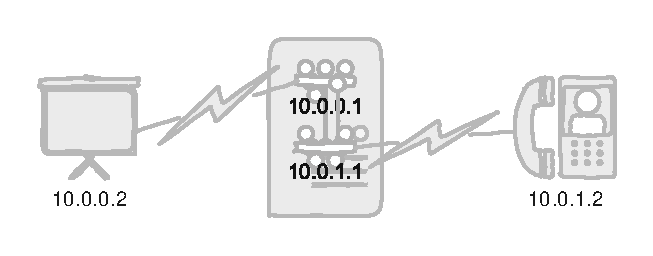
\includegraphics[width=0.6\textwidth]{exp_env.pdf}
  \caption{差错保护模块设计框架}
  \label{fig:exp_env}
\end{figure}

基本测试平台如图\ref{fig:exp_env}所示。为了对网络流量进行控制并检测网络利用情况,我们用一台具有双无线网卡的PC作为网络基站,建立两个处于不同网段(10.0.0.X 和10.0.1.X)的无线网络。视频通话终端是安装了TVphone应用的手机和连接了电视盒子的电视,并分别连接两个无线网络。由于手机和电视处于不同网段,所有通信必须通过PC基站进行中转,我们就可以在PC基站上使用流量控制软件进行不同网络状况的模拟,如丢包、延迟等。


\subsection{结果分析}
%\textcolor{red}{目前本系统的核心算法和界面都还在最后准备中,最终结果分析会在系统完成后添加。预计时间为四月底。}

\begin{figure}[htbp]
  \begin{subfigure}[b]{0.5\textwidth}
    \centering
    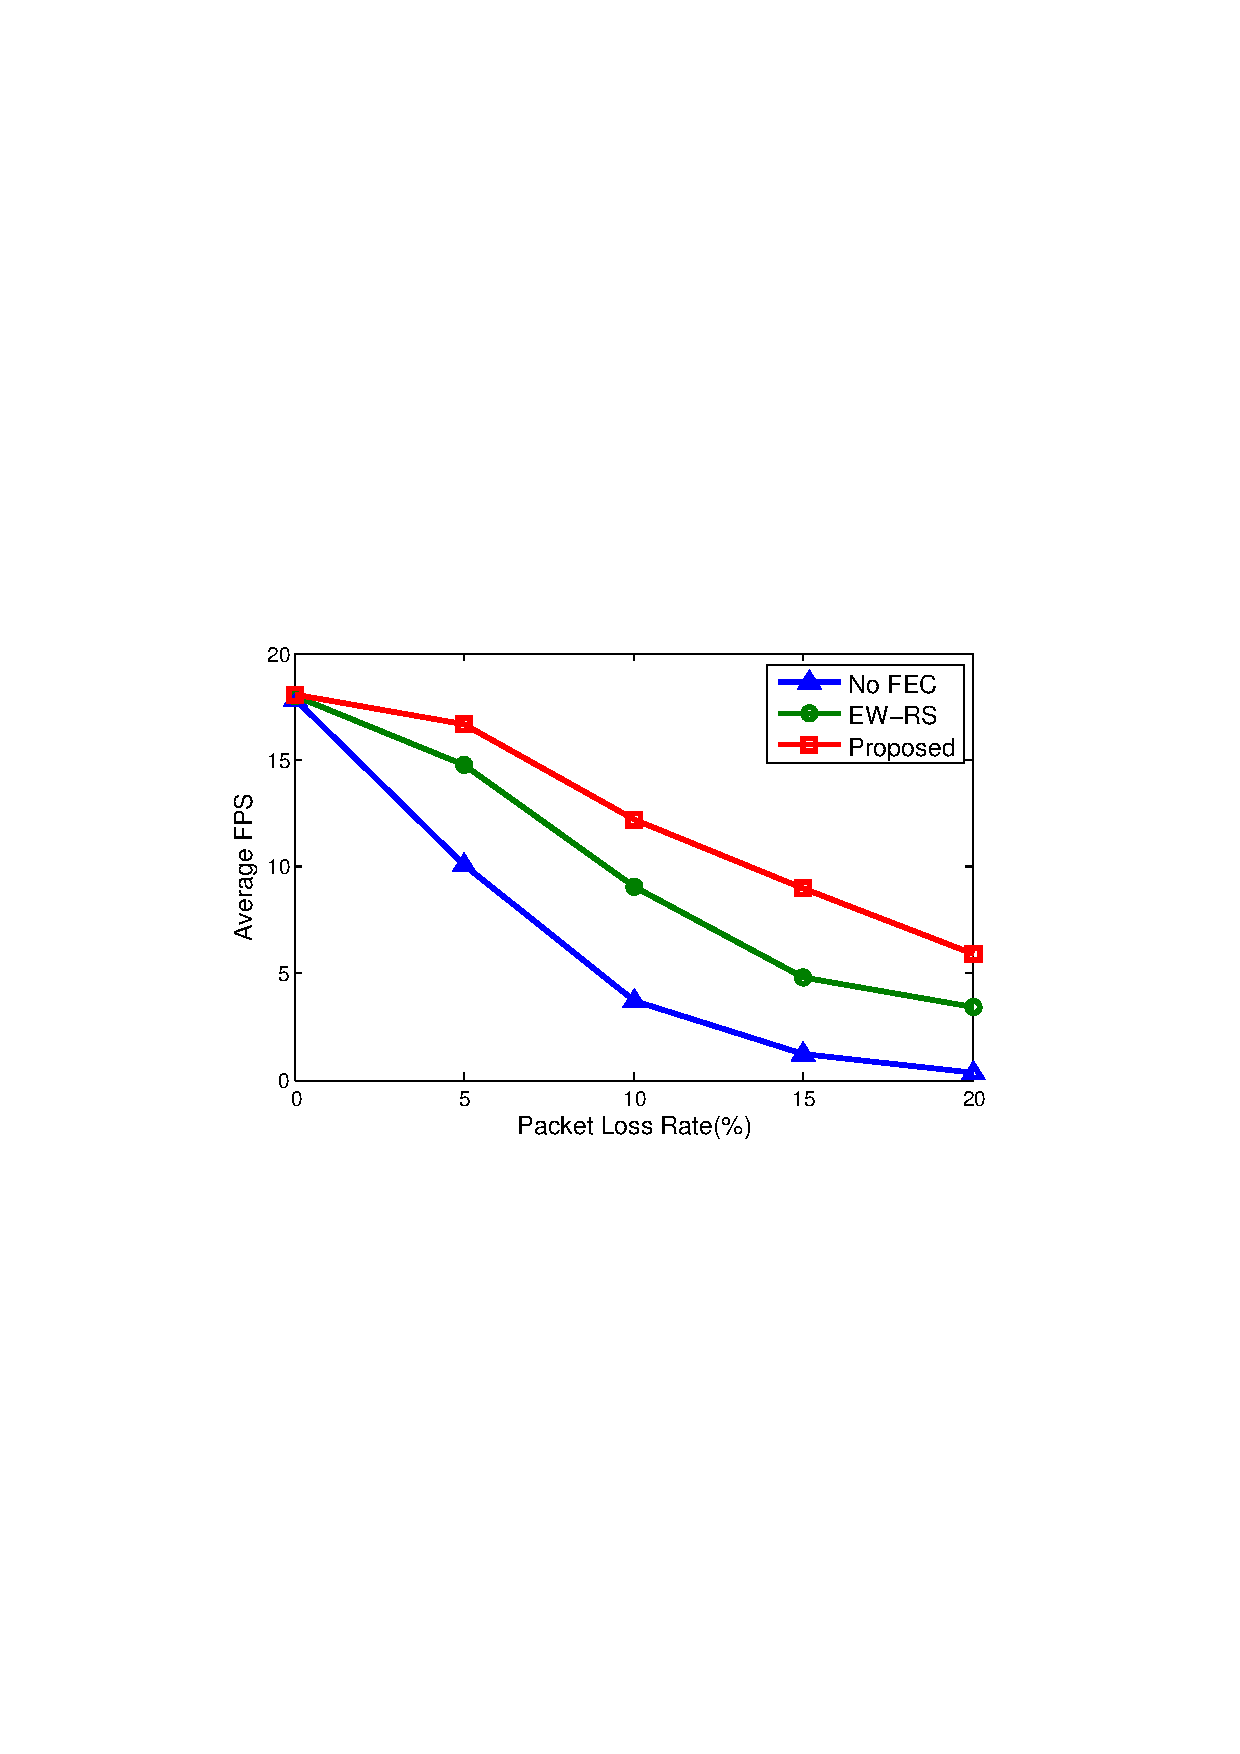
\includegraphics[scale=0.5]{tv_fps.pdf}
    \caption{帧率}
    \label{pic:tv_fps}
  \end{subfigure}
  \begin{subfigure}[b]{0.5\textwidth}
    \centering
    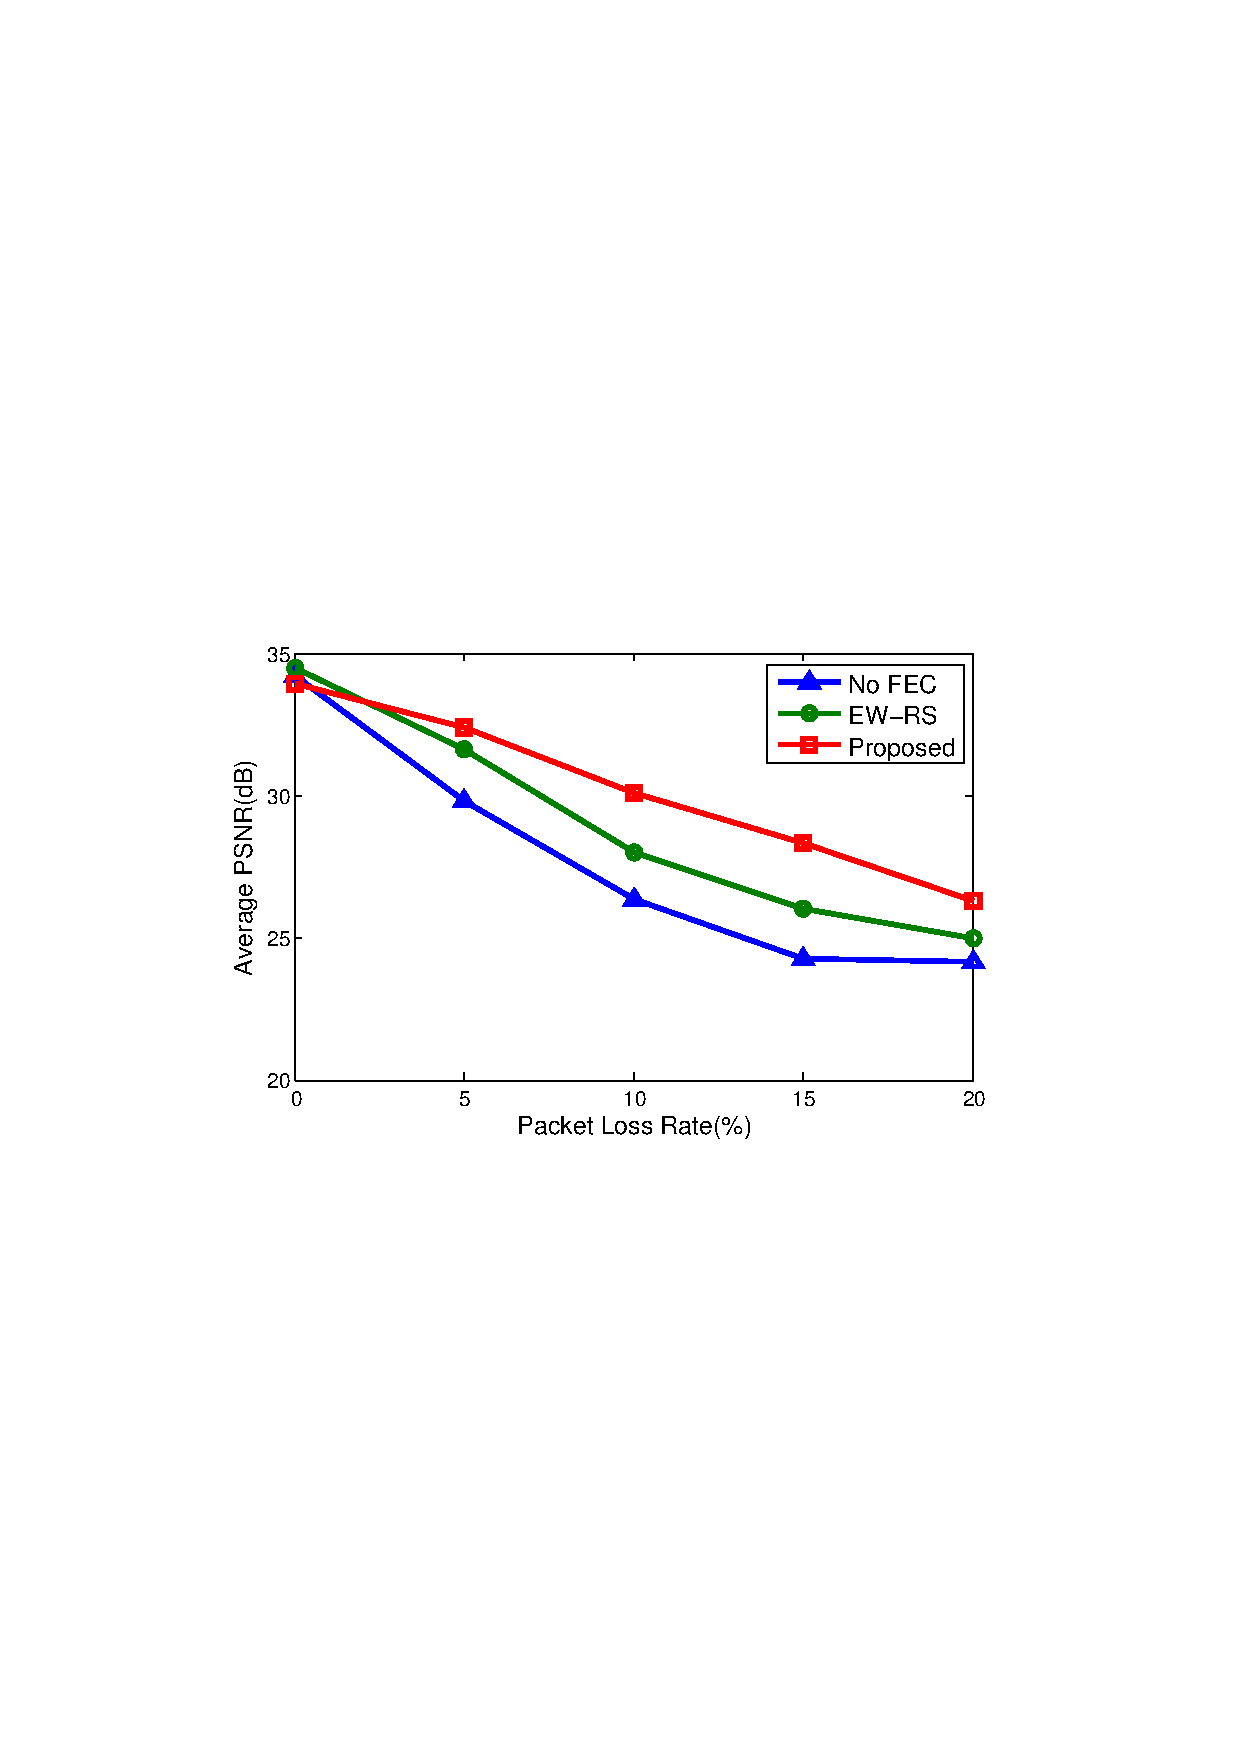
\includegraphics[scale=0.5]{tv_psnr.pdf}
    \caption{平均PSNR}
    \label{pic:tv_psnr}
  \end{subfigure}
  \caption{不同丢包率下系统表现}
  \label{fig:tv_loss}
\end{figure}

\begin{figure}[htbp]
  \centering
  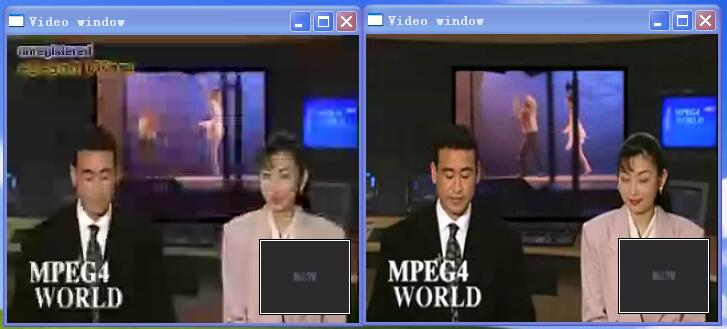
\includegraphics[width=0.9\textwidth]{exp_video.jpg}
  \caption{视频播放效果对比}
  \label{fig:exp_video}
\end{figure}

我们首先在不限制带宽的情况下,通过模拟不同的网络丢包率测试原始Linphone和TVphone对丢包的容错能力。在测试指标中,帧率(frame per second)体现了系统成功解码视频帧的能力,而平均PSNR则更精确地分析了视频画面的效果。从图 \ref{fig:tv_loss} 可以看出,由于增加了差错保护模块,我们的算法在有丢包情况下,也基本完全恢复了所有数据包,通话质量没有明显变化。而Linphone由于在丢包情况下大量视频帧无法解码,因而帧率随丢包率升高逐渐降低。同时由于帧率降低以及解码过程中由于丢包引入的画面失真,使得整体的PSNR都下降明显。图 \ref{fig:exp_video} 截取了两个系统运行中的画面,从中可以看到,左侧的Linphone通话画面画质较差,而且存在丢包造成的马赛克,与TVphone形成鲜明对比。

\section{本章小结}
为了使我们在前两章中提出的算法能够更好地服务于现实,落实到实际应用中,我们基于真实平台实现了这些算法。为此,我们调研了一个开源视频通话软件,对其整体架构、各部分模块的具体实现、底层算法都进行了总结和梳理。以此为基础,我们将新的算法实现为独立模块植入原有系统中,解决了一系列代码实现和软件兼容问题,成功升级了该视频通话软件的内核,提高了其视频传输的质量。为了拓展高清视频通话的应用场景,我们还重新设计的该系统的用户界面,将其移植到大屏幕的电视盒子上,创造了一种新的高清视频通话体验。实验表明,我们的应用明显提升了视频通话的质量。
